\documentclass[12pt]{standalone}

\usepackage{tikz}

\usetikzlibrary{decorations.markings}
\usetikzlibrary{math}

\begin{document}
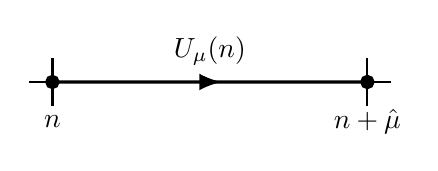
\begin{tikzpicture}

% Position settings
\tikzmath{
    \XLeft = -2;
    \XRight = 2;
    \YShift = 0.3;
}

% Draws line
\draw [black, very thick, fill] (\XLeft,0) circle (2pt) -- (\XRight,0) circle (2pt);
\draw [black, very thick, fill,
    decoration={markings, mark=at position 1 with {\arrow[black,scale=1.25,xshift=3.33333pt]{latex}}},
    postaction={decorate}] 
    (0,0) node[above=2pt] {$U_\mu(n)$};

% Draws additional lines
\draw [black, thick] (\XLeft,-\YShift) -- (\XLeft,\YShift);
\draw [black, thick] (\XRight,-\YShift) -- (\XRight,\YShift);
\draw [black, thick] (\XLeft-\YShift,0) -- (\XLeft,0) node [below=8.5pt] {$n$};
\draw [black, thick] (\XRight,0) node [below=6pt] {$n+\hat{\mu}$} -- (\XRight+\YShift,0);

% \draw [black] (\XLeft-0.5,-0.5) -- (\XRight+0.5,-0.5);



\end{tikzpicture}
\end{document}
